\documentclass[11pt,oneside]{article}
\usepackage[paperwidth=6.5in,paperheight=9.5in,margin=.72in]{geometry}
\usepackage{fontspec}
\setmainfont{lmroman10-regular.otf}[BoldFont=lmroman10-bold.otf,ItalicFont=lmroman10-italic.otf,BoldItalicFont=lmroman10-bolditalic.otf,SmallCapsFont=lmromancaps10-regular.otf]
\usepackage{amsmath,amssymb,graphicx,tikz,microtype,needspace}
\usepackage[unicode,hidelinks]{hyperref}
\hypersetup{pdftitle={Drei Fragmente über elliptische Modulfunctionen und Frickes Bemerkungen},pdfauthor={Carl Friedrich Gauss; Fricke}}
\newcommand{\SourceLeaf}[1]{\hypertarget{native-#1}{}}
\newcommand{\BareRoot}[1]{\mathord{\surd}#1}
\renewcommand{\thefootnote}{*)}
\setlength{\parindent}{1.2em}
\setlength{\emergencystretch}{1.4em}
\widowpenalty=10000\clubpenalty=10000\raggedbottom
\newcommand{\StepDown}[2]{\raisebox{-#1em}{$\displaystyle #2$}}
\begin{document}
\SourceLeaf{106}
\begin{center}\textbf{[DREI FRAGMENTE ÜBER ELLIPTISCHE MODULFUNCTIONEN.]}\end{center}
\begin{center}\rule{1.5cm}{.4pt}\end{center}
\begin{center}[1.]\end{center}

Ist
\[
\frac{n}{m}=\frac{\mu(1-2e^{-M\pi}+2e^{-4M\pi}-2e^{-9M\pi}+\cdots)^2}{\mu(1+2e^{-M\pi}+2e^{-4M\pi}+2e^{-9M\pi}+\cdots)^2},
\]
so kann man statt $M$ setzen
\[
\frac{1}{2ai}\StepDown{.75}{+\frac{1}{2bi}}\StepDown{1.5}{+\frac{1}{2ci}}\StepDown{2.25}{+\frac{1}{2di}}\StepDown{3}{+\frac{1}{2ei}}\StepDown{3.75}{+\text{etc.}+\frac{1}{M},}
\]
wo $a,b,c,d,e$ u.\,s.\,w. eine beliebige ungerade Menge ganzer reeller Zahlen bedeuten; oder auch
\[
\frac{pM+2qi}{r+2sMi}=\frac{M+2(qr-psMM)i}{rr+4ssMM},
\]
wo $p,q,r,s$ beliebige, der Bedingung
\[
pr+4qs=1
\]
Genüge leistende ganze reelle Zahlen sind.

\begin{center}\rule{3cm}{.4pt}\end{center}
\SourceLeaf{107}
\begin{center}[2.]\end{center}
\begin{center}\textbf{DIE REDUCTION VON $pM$, $qM$, $rM$ AUF DIE EINFACHSTE FORM.}\end{center}

Es sei $M=\dfrac{\alpha+\beta i}{\delta-\gamma i}$, wo $\alpha$, $\beta$, $\gamma$, $\delta$ ganze reelle Zahlen und Zähler und Nenner ohne gemeinschaftlichen Factor. Man setze
\[
\begin{gathered}
\alpha\alpha+\beta\beta=A,\qquad \alpha\gamma+\beta\delta=B,\qquad \gamma\gamma+\delta\delta=C,\\
\alpha\delta-\beta\gamma=\BareRoot{(AC-BB)}=D.
\end{gathered}
\]
Man suche die einfachste Form des Determinanten $-DD$, welche der Form $(A,B,C)$ aequivalent ist; sie sei $(a,b,c)$.

Dann lassen sich die Functionen von $M$ auf Functionen von
\[
\frac{D+bi}{a}
\]
zurückführen. Der Algorithmus ist dieser
\[
\begin{array}{ccc}
\dfrac{D+Bi}{A}=M,&DD+BB=AA',&B+B'=hA',\\[4pt]
\dfrac{D+B'i}{A'}=M',&DD+B'B'=A'A'',&B'+B''=h'A'',\\[4pt]
\dfrac{D+B''i}{A''}=M'',&DD+B''B''=A''A''',&B''+B'''=h''A''',
\end{array}
\]
\begin{center}.\quad .\quad .\quad .\quad .\quad .\quad .\quad .\quad .\quad .\quad .\quad .\quad .\quad .\quad .\quad .\quad .\quad .\quad .\quad .\quad .\end{center}
\[
\begin{array}{rl}
\BareRoot{\dfrac{D+Bi}{A}}\cdot pM=pM'&\text{für gerades }h,\\[4pt]
{}=qM'&\text{für ungerades }h,\\[5pt]\hline\\[-6pt]
\varepsilon^h\BareRoot{\dfrac{D+Bi}{A}}\cdot qM=rM',&\varepsilon=\sqrt{i},\\[5pt]\hline\\[-6pt]
\BareRoot{\dfrac{D+Bi}{A}}\cdot rM=qM'&\text{für gerades }h,\\[4pt]
{}=pM'&\text{für ungerades }h.
\end{array}
\]

Wenn man aus $h$, $h'$, $h''$ u.\,s.\,w. die Transformation von $(A,B,A')$ in $(a,b,c)$ ableitet, so werden deren Elemente (ob sie gerade oder ungerade sind) entscheiden, welche Function von $\dfrac{D+bi}{a}$ mit der gegebnen von $M$ so zusammen\SourceLeaf{108}hängt, dass letztere in
\[
\varepsilon^H\BareRoot{\left(\dfrac{D+Bi}{A}\cdot\dfrac{D+B'i}{A'}\cdot\dfrac{D+B''i}{A''}\cdots\right)}
\]
multiplicirt werden muss.

Wo $M$ nicht rational ist, mag man $D=-1$ setzen und den Algorithmus ebenso bilden; nemlich, wenn $M=g+hi$, so geht man von der Form $\left(\dfrac1g,\dfrac hg,\dfrac{gg+hh}{g}\right)$ (Det. $-1$) aus, sucht ihre Aequivalente etc.

\begin{center}\rule{3cm}{.4pt}\end{center}
\begin{center}[3.]\end{center}
\[
\begin{aligned}
pt&=1+2e^{-\pi t}+2e^{-4\pi t}+2e^{-9\pi t}+\text{etc.}\\
qt&=1-2e^{-\pi t}+2e^{-4\pi t}-2e^{-9\pi t}+\text{etc.}\\
rt&=2e^{-\frac14\pi t}+2e^{-\frac94\pi t}+2e^{-\frac{25}4\pi t}+\text{etc.}
\end{aligned}
\]

Um die Gleichung
\[
\frac{qt}{pt}=A
\]
aufzulösen, setze man $AA=\dfrac nm$ und suche das a.-g. Mittel zwischen $m$ und $n$; es sei dasselbe $=\mu$. Man suche ferner das a.-g. Mittel zwischen $m$ und $\BareRoot{(mm-nn)}$ oder, was dasselbe ist, zwischen $(m+n)$ und $(m-n)$; dieses sei $=\lambda$. Man hat dann $t=\dfrac\mu\lambda$.

Man erhält so nur Einen Werth von $t$; sämmtliche andere werden dann in der Formel
\[
\frac{\alpha t-2\beta i}{\delta-2\gamma ti}
\]
enthalten sein, wo $\alpha$, $\beta$, $\gamma$, $\delta$ alle ganzen Zahlen bedeuten, die der Gleichung:
\[
\alpha\delta-4\beta\gamma=1
\]
Genüge leisten.

Um aus $A$ abzuleiten
\[
B=\dfrac{q\!\left(\frac13t\right)}{p\!\left(\frac13t\right)},
\]
\SourceLeaf{109}ist eine biquadratische Gleichung aufzulösen:
\[
(B-A)^4=4(A-A^3)(B-B^3),
\]
oder
\[
(1-AB)^4=(1-A^4)(1-B^4).
\]

Den vier Wurzeln correspondiren $\frac13t$, $\frac13t+\frac23i$, $\frac13t+\frac43i$, $3t$.

Für $A=\frac12$ suche man zwei a.-g. Mittel
\[
\begin{aligned}
m&=4, & n&=1\\
\mu&=2{,}2430340, &\lambda&=3{,}9364917.
\end{aligned}
\]
Also
\[
\begin{array}{rl}
t=&0{,}56983,\\
\log t=&9{,}7557537,\\
\log(\pi\log e)=&0{,}1349342,\\\hline
&9{,}8906879,\\
\log e^{-\pi t}=&-0{,}7774777,\\
{}=&9{,}2225223,\\
pt=&1{,}33540375,\\
qt=&0{,}66770187.
\end{array}
\]
\begin{center}\rule{3cm}{.4pt}\end{center}

\clearpage
\enlargethispage{2pt}

\begin{center}\textbf{BEMERKUNGEN ZU DEN FRAGMENTEN\\ ÜBER ELLIPTISCHE MODULFUNCTIONEN.}\end{center}

Der durch den Algorithmus des arithmetisch-geometrischen Mittels gegebene Ansatz, vermöge dessen sich \textsc{Gauss} den Zugang zur Theorie der elliptischen Functionen und der zugehörigen Modulfunctionen gebahnt hat, brachte es mit sich, dass bei \textsc{Gauss} (entgegen der neuerdings für gewöhnlich befolgten Entwicklungsweise) die Modulfunctionen den allgemeinen elliptischen Functionen voranstehen. Dieser Standpunkt ist insofern der natürliche, als die Modulfunctionen Functionen einer einzigen Variabelen bez. zweier homogener Variabelen sind, während die allgemeinen elliptischen Functionen von zwei Argumenten bez. von drei homogenen Argumenten abhängen.

Der fragliche Algorithmus in richtiger Allgemeinheit ist in Art. 12\footnote{Hier und weiterhin sind die Artikel der aus dem Nachlass herausgegebenen Abhandlung über das arithmetisch-geometrische Mittel (ges. Werke III p. 361--403) gemeint.} definirt. Aus drei zunächst reellen \SourceLeaf{110}Grössen $a$, $b$, $c$ werden die beiden Mittel $M(a,b)$ und $M(a,c)$ abgeleitet und in ihrer Abhängigkeit vom gegebenen Tripel $a$, $b$, $c$ studirt.

Zwei Gesichtspunkte werden alsdann für die \textsc{Gauss}'sche Entwicklung fundamental. Erstlich handelt es sich um den auch in der späteren Entwicklung der Theorie der elliptischen Functionen so bedeutungsvollen Gedanken der \emph{Inversion}, d.\,i. um das Problem, die ursprünglich gegebenen $a$, $b$, $c$ in ihrer Abhängigkeit von $M(a,b)$ und $M(a,c)$ aufzufassen. Andrerseits wird beim Ausbau dieser Auffassung die Annahme der $a$, $b$, $c$ bez. $M(a,b)$, $M(a,c)$ als \emph{complexer Variabeler} natürlich bez. nothwendig.

In erster Hinsicht ist es ein wichtiges Ergebniss, dass \textsc{Gauss} bereits in den neunziger Jahren des vorigen Jahrhunderts die Reihenentwicklungen für die Nullwerthe der drei geraden $\vartheta$-Functionen gekannt hat. Die hierbei angewendete Überlegung (s. Art. 16) ist sowohl im Hinblick auf die Erfassung des wahren Zieles der Untersuchung, wie auch wegen der im einzelnen befolgten Schlussweisen höchst bemerkenswerth.

Die Zulassung complexer Variabelen erschien namentlich wegen der Entwicklungen in Art. 17 geboten. Es werden daselbst die Grundformeln für die lineare Transformation der $\vartheta$-Nullwerthe aufgestellt. Von hier aus aber hat \textsc{Gauss} eine Reihe wichtiger Grundsätze der Theorie der Modulfunctionen erkannt, die erst in neuerer Zeit allgemein zugänglich geworden sind.

Man wolle in dieser Hinsicht erstlich die Angaben des Art. 17 vergleichen, demnächst aber die vorstehend abgedruckten Fragmente. Die Grösse $t$ des Fragmentes [3] hängt mit dem Periodenquotienten $\omega$ der neueren Theorie vermöge der Gleichung $\omega = it$ zusammen. Die Erzeugenden der Gruppe aller linearen Periodentransformationen werden daraufhin:

\[
t' = t+i, \qquad t' = \frac1t.
\]

Mit der Zusammensetzung der übrigen Substitutionen der genannten Gruppe aus diesen Erzeugenden hat sich \textsc{Gauss} wiederholt beschäftigt. Neben den Angaben des Fragmentes [1] sei noch die Formel erwähnt

\[
\frac{[\alpha,\beta,\ldots,\nu]\theta+[\beta,\gamma,\ldots,\nu]i}{-i[\alpha,\beta,\ldots,\mu]\theta+[\beta,\gamma,\ldots,\mu]},
\]
welche sich in einem »Cereri Palladi Junoni sacrum, Febr. 1805« betitelten Hefte findet. Als Beispiele sind ebenda die Kettenbruchentwicklungen der beiden Substitutionen gegeben:

\[
\frac{128\theta+37i}{-45i\theta+13}, \qquad \frac{121\theta+36i}{-84i\theta+25}.
\]

Sowohl zur Erläuterung der Kettenbruchentwicklung der Substitutionen als auch zum Vollzug functionentheoretischer Schlüsse hat sich \textsc{Gauss} derjenigen geometrischen Darstellungsweise bedient, welche zur Grundlage der neueren Theorie der Modulfunctionen geworden ist. In dem eben schon erwähnten Hefte hat \textsc{Gauss} die hierneben wiedergegebene Figur gezeichnet. Da sich daneben die erwähnten Kettenbruchentwicklungen von Substitutionen finden, so wird \textsc{Gauss} die Figur als Mittel zur Veranschaulichung dieser Kettenbruchentwicklungen benutzt haben. In der That hat man ja hier den Beginn des wohlbekannten Netzes der Kreisbogendreiecke, welches der Theorie der Modulfunctionen zu Grunde liegt.

\begin{center}\resizebox{9.7cm}{!}{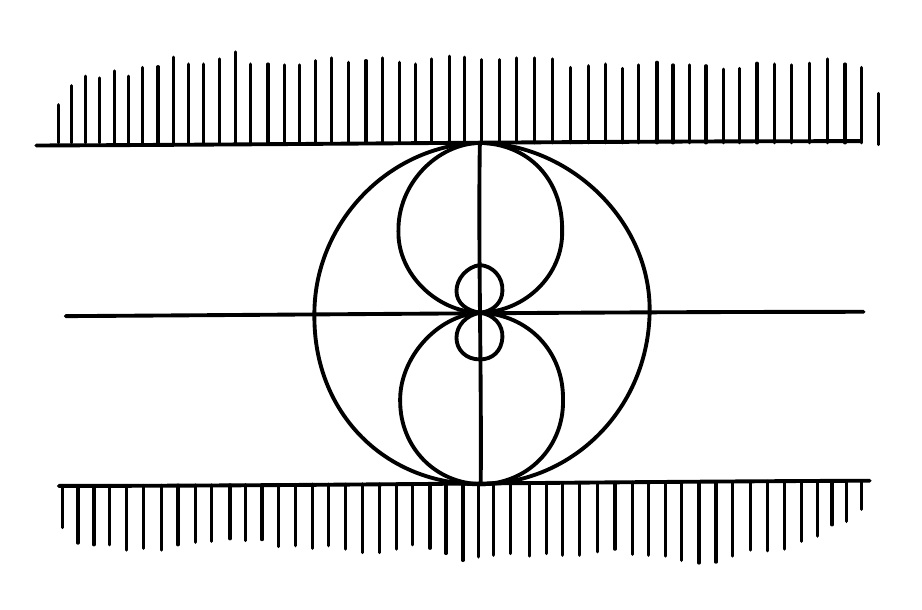
\begin{tikzpicture}[x=.011cm,y=-.011cm,line cap=round,line join=round]
\path[use as bounding box] (0,0) rectangle (1000,640);
% Hatch strokes: source-measured positions and extents; no repeated mathematical values inferred.
\draw[line width=1.15pt] (35.5,89.0) -- (35.5,133.0);
\draw[line width=1.15pt] (51.0,67.0) -- (51.0,133.0);
\draw[line width=1.15pt] (67.0,56.0) -- (67.0,133.0);
\draw[line width=1.15pt] (82.5,58.0) -- (82.5,133.0);
\draw[line width=1.15pt] (100.0,50.0) -- (100.0,133.0);
\draw[line width=1.15pt] (116.0,56.0) -- (116.0,133.0);
\draw[line width=1.15pt] (132.5,46.0) -- (132.5,133.0);
\draw[line width=1.15pt] (150.5,45.0) -- (150.5,133.0);
\draw[line width=1.15pt] (168.0,34.0) -- (168.0,133.0);
\draw[line width=1.15pt] (185.5,42.0) -- (185.5,133.0);
\draw[line width=1.15pt] (203.0,42.0) -- (203.0,133.0);
\draw[line width=1.15pt] (221.5,36.0) -- (221.5,133.0);
\draw[line width=1.15pt] (240.0,28.0) -- (240.0,133.0);
\draw[line width=1.15pt] (257.5,42.0) -- (257.5,133.0);
\draw[line width=1.15pt] (277.5,42.0) -- (277.5,133.0);
\draw[line width=1.15pt] (296.5,43.0) -- (296.5,133.0);
\draw[line width=1.15pt] (313.5,43.0) -- (313.5,133.0);
\draw[line width=1.15pt] (332.0,38.0) -- (332.0,133.0);
\draw[line width=1.15pt] (350.5,35.0) -- (350.5,133.0);
\draw[line width=1.15pt] (370.0,40.0) -- (370.0,133.0);
\draw[line width=1.15pt] (390.5,38.0) -- (390.5,133.0);
\draw[line width=1.15pt] (409.5,35.0) -- (409.5,133.0);
\draw[line width=1.15pt] (429.0,40.0) -- (429.0,133.0);
\draw[line width=1.15pt] (448.0,42.0) -- (448.0,133.0);
\draw[line width=1.15pt] (466.0,36.0) -- (466.0,133.0);
\draw[line width=1.15pt] (486.5,33.0) -- (486.5,133.0);
\draw[line width=1.15pt] (504.5,34.0) -- (504.5,133.0);
\draw[line width=1.15pt] (523.5,37.0) -- (523.5,133.0);
\draw[line width=1.15pt] (544.5,37.0) -- (544.5,133.0);
\draw[line width=1.15pt] (564.5,35.0) -- (564.5,133.0);
\draw[line width=1.15pt] (585.5,35.0) -- (585.5,133.0);
\draw[line width=1.15pt] (606.0,36.0) -- (606.0,133.0);
\draw[line width=1.15pt] (626.5,46.0) -- (626.5,133.0);
\draw[line width=1.15pt] (647.0,44.0) -- (647.0,133.0);
\draw[line width=1.15pt] (667.5,42.0) -- (667.5,133.0);
\draw[line width=1.15pt] (687.0,47.0) -- (687.0,133.0);
\draw[line width=1.15pt] (705.5,43.0) -- (705.5,133.0);
\draw[line width=1.15pt] (726.5,40.0) -- (726.5,133.0);
\draw[line width=1.15pt] (745.0,43.0) -- (745.0,133.0);
\draw[line width=1.15pt] (764.0,43.0) -- (764.0,133.0);
\draw[line width=1.15pt] (783.0,44.0) -- (783.0,133.0);
\draw[line width=1.15pt] (803.5,48.0) -- (803.5,133.0);
\draw[line width=1.15pt] (822.0,47.0) -- (822.0,133.0);
\draw[line width=1.15pt] (842.0,41.0) -- (842.0,133.0);
\draw[line width=1.15pt] (862.5,42.0) -- (862.5,133.0);
\draw[line width=1.15pt] (882.0,43.0) -- (882.0,133.0);
\draw[line width=1.15pt] (902.5,41.0) -- (902.5,133.0);
\draw[line width=1.15pt] (923.5,36.0) -- (923.5,133.0);
\draw[line width=1.15pt] (943.5,42.0) -- (943.5,133.0);
\draw[line width=1.15pt] (962.5,46.0) -- (962.5,133.0);
\draw[line width=1.15pt] (982.0,76.0) -- (982.0,135.0);
\draw[line width=1.15pt] (40.0,529.0) -- (40.0,577.0);
\draw[line width=1.15pt] (58.0,528.9) -- (58.0,595.0);
\draw[line width=1.15pt] (76.5,528.8) -- (76.5,597.0);
\draw[line width=1.15pt] (94.5,528.6) -- (94.5,597.0);
\draw[line width=1.15pt] (114.5,528.5) -- (114.5,603.0);
\draw[line width=1.15pt] (133.5,528.4) -- (133.5,601.0);
\draw[line width=1.15pt] (154.5,528.3) -- (154.5,603.0);
\draw[line width=1.15pt] (173.5,528.1) -- (173.5,597.0);
\draw[line width=1.15pt] (194.0,528.0) -- (194.0,594.0);
\draw[line width=1.15pt] (212.5,527.9) -- (212.5,593.0);
\draw[line width=1.15pt] (233.5,527.8) -- (233.5,590.0);
\draw[line width=1.15pt] (251.5,527.6) -- (251.5,592.0);
\draw[line width=1.15pt] (270.5,527.5) -- (270.5,591.0);
\draw[line width=1.15pt] (290.0,527.4) -- (290.0,599.0);
\draw[line width=1.15pt] (309.5,527.3) -- (309.5,598.0);
\draw[line width=1.15pt] (328.5,527.1) -- (328.5,601.0);
\draw[line width=1.15pt] (347.5,527.0) -- (347.5,598.0);
\draw[line width=1.15pt] (367.0,526.9) -- (367.0,602.0);
\draw[line width=1.15pt] (386.5,526.8) -- (386.5,606.0);
\draw[line width=1.15pt] (406.5,526.6) -- (406.5,606.0);
\draw[line width=1.15pt] (425.5,526.5) -- (425.5,602.0);
\draw[line width=1.15pt] (444.5,526.4) -- (444.5,597.0);
\draw[line width=1.15pt] (464.5,526.3) -- (464.5,601.0);
\draw[line width=1.15pt] (483.0,526.1) -- (483.0,607.0);
\draw[line width=1.15pt] (502.5,526.0) -- (502.5,615.0);
\draw[line width=1.15pt] (520.5,525.9) -- (520.5,611.0);
\draw[line width=1.15pt] (537.5,525.8) -- (537.5,609.0);
\draw[line width=1.15pt] (557.5,525.7) -- (557.5,607.0);
\draw[line width=1.15pt] (579.5,525.5) -- (579.5,610.0);
\draw[line width=1.15pt] (598.5,525.4) -- (598.5,607.0);
\draw[line width=1.15pt] (617.5,525.3) -- (617.5,609.0);
\draw[line width=1.15pt] (637.0,525.1) -- (637.0,609.0);
\draw[line width=1.15pt] (657.5,525.0) -- (657.5,605.0);
\draw[line width=1.15pt] (678.0,524.9) -- (678.0,602.0);
\draw[line width=1.15pt] (698.0,524.8) -- (698.0,608.0);
\draw[line width=1.15pt] (717.0,524.6) -- (717.0,609.0);
\draw[line width=1.15pt] (736.0,524.5) -- (736.0,610.0);
\draw[line width=1.15pt] (754.5,524.4) -- (754.5,615.0);
\draw[line width=1.15pt] (775.0,524.3) -- (775.0,618.0);
\draw[line width=1.15pt] (794.5,524.1) -- (794.5,617.0);
\draw[line width=1.15pt] (814.0,524.0) -- (814.0,610.0);
\draw[line width=1.15pt] (834.0,523.9) -- (834.0,603.0);
\draw[line width=1.15pt] (854.0,523.7) -- (854.0,604.0);
\draw[line width=1.15pt] (874.0,523.6) -- (874.0,602.0);
\draw[line width=1.15pt] (893.0,523.5) -- (893.0,593.0);
\draw[line width=1.15pt] (911.5,523.4) -- (911.5,587.0);
\draw[line width=1.15pt] (928.5,523.3) -- (928.5,574.0);
\draw[line width=1.15pt] (945.5,523.2) -- (945.5,570.0);
\draw[line width=1.15pt] (962.5,523.0) -- (962.5,556.0);
\draw[line width=1.4pt] (522.0,133.0) .. controls (626.0,134.0) and (719.0,223.0) .. (718.0,327.0) .. controls (717.0,438.0) and (631.0,526.0) .. (523.0,527.0) .. controls (414.0,528.0) and (330.0,446.0) .. (331.0,332.0) .. controls (330.0,226.0) and (417.0,135.0) .. (522.0,133.0) -- cycle;
\draw[line width=1.4pt] (522.0,133.0) .. controls (577.0,134.0) and (618.0,174.0) .. (617.0,235.0) .. controls (618.0,285.0) and (575.0,328.0) .. (522.0,329.0) .. controls (472.0,328.0) and (427.0,284.0) .. (428.0,235.0) .. controls (427.0,180.0) and (473.0,134.0) .. (522.0,133.0) -- cycle;
\draw[line width=1.4pt] (522.0,329.0) .. controls (578.0,331.0) and (619.0,374.0) .. (618.0,430.0) .. controls (619.0,484.0) and (577.0,527.0) .. (523.0,527.0) .. controls (470.0,526.0) and (430.0,484.0) .. (430.0,431.0) .. controls (429.0,382.0) and (472.0,332.0) .. (522.0,329.0) -- cycle;
\draw[line width=1.4pt] (522.0,274.0) .. controls (537.0,275.0) and (549.0,288.0) .. (548.0,304.0) .. controls (548.0,317.0) and (537.0,328.0) .. (522.0,329.0) .. controls (507.0,327.0) and (495.0,318.0) .. (495.0,304.0) .. controls (495.0,290.0) and (507.0,276.0) .. (522.0,274.0) -- cycle;
\draw[line width=1.4pt] (522.0,329.0) .. controls (538.0,331.0) and (549.0,343.0) .. (548.0,358.0) .. controls (547.0,373.0) and (537.0,383.0) .. (522.0,383.0) .. controls (506.0,383.0) and (495.0,372.0) .. (495.0,358.0) .. controls (495.0,344.0) and (506.0,332.0) .. (522.0,329.0) -- cycle;
\draw[line width=1.4pt] (10.0,136.0) .. controls (300.0,135.0) and (640.0,131.0) .. (962.0,131.0);
\draw[line width=1.4pt] (44.0,333.0) .. controls (360.0,331.0) and (680.0,328.0) .. (965.0,328.0);
\draw[line width=1.4pt] (36.0,529.0) .. controls (320.0,529.0) and (680.0,524.0) .. (972.0,523.0);
\draw[line width=1.4pt] (522.0,133.0) .. controls (520.0,260.0) and (524.0,390.0) .. (523.0,527.0);
\end{tikzpicture}
}\end{center}

Dass \textsc{Gauss} das hierbei in Betracht kommende »Princip der symmetrischen Vervielfältigung von Kreisbogendreiecken« allgemein aufgefasst hat, ja dass ihm so\SourceLeaf{111}gar der Charakter der »natürlichen Grenze« eines so zu gewinnenden Dreiecksnetzes nicht verborgen blieb, geht auch aus der zweiten hier zum Abdruck kommenden Zeichnung hervor, welche sich im Nachlass auf einem

\begin{center}\resizebox{12.3cm}{!}{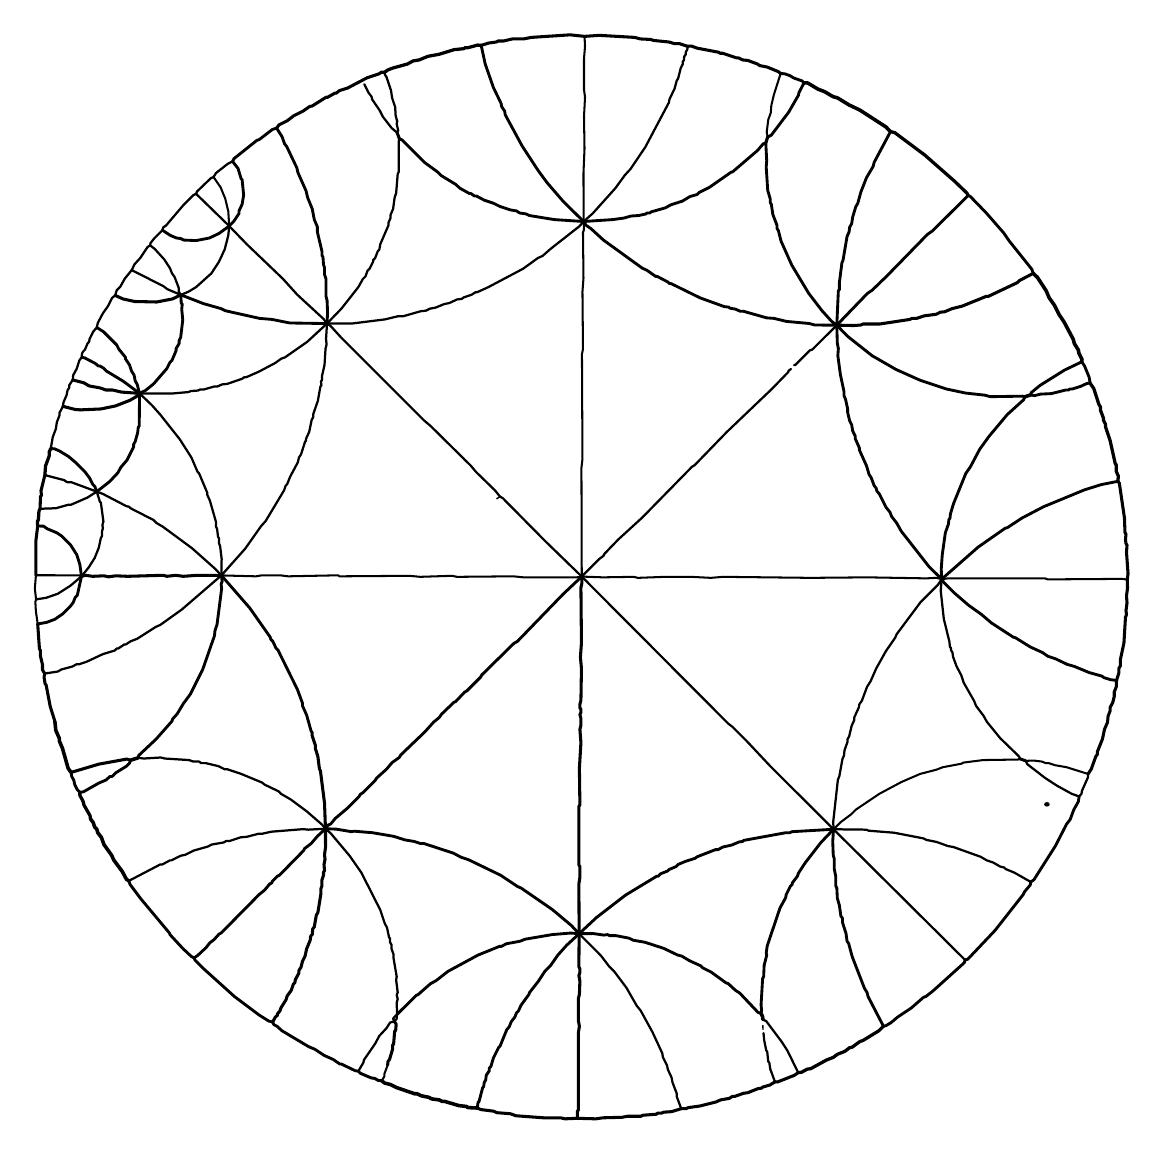
\begin{tikzpicture}[x=.0065cm,y=-.0065cm,line cap=round,line join=round]
\path[use as bounding box] (-12,-12) rectangle (2155,2137);
% Editable source-measured arc segment 1.
\draw[line width=1.1055pt] (1076.000,5.000) -- (1048.000,2.000) -- (972.000,7.000) -- (957.000,10.000) -- (935.000,10.000) -- (918.000,14.000) -- (907.000,14.000) -- (904.000,16.000) -- (889.000,18.000) -- (874.077,22.538);
% Editable source-measured arc segment 2.
\draw[line width=1.1055pt] (1076.000,5.000) -- (1105.000,3.000) -- (1174.000,7.000) -- (1185.000,10.000) -- (1205.000,11.000) -- (1211.000,13.000) -- (1241.000,16.000) -- (1251.000,19.000) -- (1261.000,19.000) -- (1277.000,24.385);
% Editable source-measured arc segment 3.
\draw[line width=0.7370pt] (1076.000,5.000) -- (1077.000,24.000) -- (1075.000,49.000) -- (1075.000,109.000) -- (1077.000,124.000) -- (1075.000,162.000) -- (1076.000,224.000) -- (1074.000,272.000) -- (1074.213,366.745);
% Editable source-measured arc segment 4.
\draw[line width=1.1781pt] (874.077,22.538) -- (867.000,22.000) -- (849.000,27.000) -- (843.000,27.000) -- (840.000,29.000) -- (821.000,31.000) -- (792.000,40.000) -- (770.000,44.000) -- (753.000,51.000) -- (741.000,53.000) -- (730.000,59.000) -- (701.000,67.000) -- (691.000,71.000) -- (685.692,75.154);
% Editable source-measured arc segment 5.
\draw[line width=1.0318pt] (874.077,22.538) -- (882.000,59.000) -- (898.000,105.000) -- (913.000,136.000) -- (914.000,142.000) -- (920.000,151.000) -- (921.000,158.000) -- (954.000,219.000) -- (986.000,268.000) -- (1003.000,291.000) -- (1034.000,327.000) -- (1074.213,366.745);
% Editable source-measured arc segment 6.
\draw[line width=1.1055pt] (1277.000,24.385) -- (1285.000,24.000) -- (1296.000,28.000) -- (1338.000,36.000) -- (1341.000,38.000) -- (1346.000,38.000) -- (1373.000,47.000) -- (1377.000,47.000) -- (1385.000,51.000) -- (1395.000,52.000) -- (1414.000,59.000) -- (1418.000,62.000) -- (1433.000,65.000) -- (1455.000,74.000) -- (1459.167,77.667);
% Editable source-measured arc segment 7.
\draw[line width=0.8096pt] (1277.000,24.385) -- (1277.000,30.000) -- (1274.000,36.000) -- (1274.000,40.000) -- (1271.000,44.000) -- (1270.000,52.000) -- (1268.000,54.000) -- (1268.000,59.000) -- (1264.000,67.000) -- (1259.000,87.000) -- (1256.000,92.000) -- (1252.000,107.000) -- (1242.000,128.000) -- (1241.000,134.000) -- (1195.000,221.000) -- (1166.000,264.000) -- (1155.000,276.000) -- (1136.000,302.000) -- (1092.000,351.000) -- (1074.213,366.745);
% Editable source-measured arc segment 8.
\draw[line width=1.1055pt] (685.692,75.154) -- (679.000,75.000) -- (675.000,78.000) -- (651.000,86.000) -- (613.000,106.000) -- (597.000,111.000) -- (591.000,116.000) -- (588.000,116.000) -- (574.000,124.000) -- (571.000,124.000) -- (544.000,141.000) -- (539.000,142.000) -- (526.000,151.000) -- (508.000,160.000) -- (495.000,170.000) -- (479.000,178.000) -- (474.400,184.200);
% Editable source-measured arc segment 9.
\draw[line width=0.8096pt] (685.692,75.154) -- (686.000,80.000) -- (689.000,84.000) -- (698.000,111.000) -- (700.000,125.000) -- (706.000,143.000) -- (707.000,160.000) -- (710.000,171.000) -- (709.000,176.000) -- (712.000,189.000) -- (709.833,193.083);
% Editable source-measured arc segment 10.
\draw[line width=1.0318pt] (1459.167,77.667) -- (1467.000,78.000) -- (1478.000,82.000) -- (1484.000,86.000) -- (1501.000,92.000) -- (1504.786,96.000);
% Editable source-measured arc segment 11.
\draw[line width=0.7370pt] (1459.167,77.667) -- (1446.000,119.000) -- (1441.000,140.000) -- (1440.000,154.000) -- (1435.000,168.000) -- (1432.000,192.000) -- (1433.800,201.700);
% Editable source-measured arc segment 12.
\draw[line width=1.2898pt] (1504.786,96.000) -- (1512.000,96.000) -- (1532.000,108.000) -- (1545.000,113.000) -- (1562.000,123.000) -- (1570.000,125.000) -- (1593.000,139.000) -- (1614.000,149.000) -- (1665.000,182.000) -- (1673.900,191.100);
% Editable source-measured arc segment 13.
\draw[line width=1.0318pt] (1504.786,96.000) -- (1495.000,115.000) -- (1494.000,120.000) -- (1475.000,153.000) -- (1441.000,198.000) -- (1433.800,201.700);
% Editable source-measured arc segment 14.
\draw[line width=0.8096pt] (645.750,98.500) -- (654.000,115.000) -- (660.000,123.000) -- (661.000,128.000) -- (676.000,150.000) -- (682.000,162.000) -- (699.000,184.000) -- (709.833,193.083);
% Editable source-measured arc segment 15.
\draw[line width=1.0318pt] (474.400,184.200) -- (466.000,187.000) -- (440.000,207.000) -- (436.000,208.000) -- (391.000,244.000) -- (388.400,249.400);
% Editable source-measured arc segment 16.
\draw[line width=1.0318pt] (474.400,184.200) -- (485.000,201.000) -- (490.000,215.000) -- (494.000,220.000) -- (514.000,262.000) -- (516.000,271.000) -- (532.000,307.000) -- (535.000,320.000) -- (544.000,342.000) -- (548.000,363.000) -- (554.000,377.000) -- (554.000,387.000) -- (563.000,425.000) -- (563.000,433.000) -- (565.000,436.000) -- (566.000,451.000) -- (568.000,457.000) -- (568.000,470.000) -- (571.000,479.000) -- (571.000,513.000) -- (573.000,521.000) -- (574.000,545.000) -- (572.841,566.136);
% Editable source-measured arc segment 17.
\draw[line width=1.1781pt] (1673.900,191.100) -- (1682.000,193.000) -- (1741.000,237.000) -- (1799.000,288.000) -- (1823.000,311.000) -- (1825.500,315.917);
% Editable source-measured arc segment 18.
\draw[line width=1.0318pt] (1673.900,191.100) -- (1642.000,251.000) -- (1640.000,259.000) -- (1627.000,281.000) -- (1616.000,309.000) -- (1610.000,331.000) -- (1606.000,338.000) -- (1600.000,358.000) -- (1598.000,371.000) -- (1594.000,378.000) -- (1593.000,387.000) -- (1589.000,396.000) -- (1581.000,443.000) -- (1579.000,447.000) -- (1574.000,486.000) -- (1574.000,500.000) -- (1572.000,502.000) -- (1568.917,569.271);
% Editable source-measured arc segment 19.
\draw[line width=1.1055pt] (709.833,193.083) -- (714.286,205.071);
% Editable source-measured arc segment 20.
\draw[line width=1.1418pt] (1433.800,201.700) -- (1430.200,213.300);
% Editable source-measured arc segment 21.
\draw[line width=1.0318pt] (714.286,205.071) -- (719.000,207.000) -- (763.000,251.000) -- (789.000,270.000) -- (796.000,277.000) -- (824.000,294.000) -- (833.000,302.000) -- (851.000,312.000) -- (854.000,312.000) -- (861.000,317.000) -- (865.000,317.000) -- (880.000,325.000) -- (898.000,331.000) -- (910.000,337.000) -- (931.000,344.000) -- (943.000,346.000) -- (949.000,350.000) -- (962.000,352.000) -- (968.000,355.000) -- (1017.000,363.000) -- (1074.213,366.745);
% Editable source-measured arc segment 22.
\draw[line width=0.8096pt] (714.286,205.071) -- (713.000,210.000) -- (713.000,270.000) -- (711.000,274.000) -- (708.000,311.000) -- (705.000,320.000) -- (702.000,342.000) -- (697.000,354.000) -- (697.000,360.000) -- (693.000,369.000) -- (693.000,374.000) -- (677.000,411.000) -- (675.000,422.000) -- (672.000,425.000) -- (667.000,438.000) -- (663.000,442.000) -- (663.000,445.000) -- (656.000,459.000) -- (652.000,463.000) -- (648.000,474.000) -- (643.000,479.000) -- (634.000,495.000) -- (601.000,537.000) -- (572.841,566.136);
% Editable source-measured arc segment 23.
\draw[line width=1.0318pt] (1430.200,213.300) -- (1425.000,215.000) -- (1414.000,228.000) -- (1365.000,270.000) -- (1363.000,270.000) -- (1320.000,300.000) -- (1300.000,310.000) -- (1296.000,314.000) -- (1282.000,318.000) -- (1267.000,327.000) -- (1245.000,334.000) -- (1234.000,340.000) -- (1206.000,348.000) -- (1204.000,350.000) -- (1198.000,350.000) -- (1196.000,352.000) -- (1182.000,355.000) -- (1167.000,356.000) -- (1153.000,360.000) -- (1131.000,363.000) -- (1074.213,366.745);
% Editable source-measured arc segment 24.
\draw[line width=1.0318pt] (1430.200,213.300) -- (1432.000,248.000) -- (1431.000,260.000) -- (1434.000,306.000) -- (1439.000,323.000) -- (1439.000,330.000) -- (1441.000,333.000) -- (1444.000,353.000) -- (1452.000,374.000) -- (1452.000,380.000) -- (1455.000,385.000) -- (1460.000,405.000) -- (1481.000,452.000) -- (1514.000,507.000) -- (1540.000,541.000) -- (1559.000,562.000) -- (1568.917,569.271);
% Editable source-measured arc segment 25.
\draw[line width=0.8096pt] (388.400,249.400) -- (379.000,254.000) -- (356.000,272.000) -- (351.154,279.846);
% Editable source-measured arc segment 26.
\draw[line width=1.0318pt] (388.400,249.400) -- (399.000,263.000) -- (405.000,283.000) -- (407.000,285.000) -- (410.000,315.000) -- (407.000,333.000) -- (401.000,346.000) -- (401.000,351.000) -- (391.000,366.000) -- (381.743,375.543);
% Editable source-measured arc segment 27.
\draw[line width=0.8096pt] (351.154,279.846) -- (346.000,282.000) -- (319.000,308.000) -- (317.000,312.583);
% Editable source-measured arc segment 28.
\draw[line width=0.7370pt] (351.154,279.846) -- (365.000,300.000) -- (374.000,322.000) -- (380.000,347.000) -- (381.743,375.543);
% Editable source-measured arc segment 29.
\draw[line width=0.8096pt] (317.000,312.583) -- (312.000,315.000) -- (292.000,335.000) -- (258.000,375.000) -- (253.000,378.000) -- (251.231,383.769);
% Editable source-measured arc segment 30.
\draw[line width=0.8096pt] (317.000,312.583) -- (381.743,375.543);
% Editable source-measured arc segment 31.
\draw[line width=1.0318pt] (1825.500,315.917) -- (1830.000,318.000) -- (1861.000,350.000) -- (1895.000,389.000) -- (1906.000,405.000) -- (1950.000,460.000) -- (1952.769,468.077);
% Editable source-measured arc segment 32.
\draw[line width=1.0318pt] (1825.500,315.917) -- (1756.000,385.000) -- (1746.000,392.000) -- (1667.000,473.000) -- (1638.000,501.000) -- (1629.000,507.000) -- (1568.917,569.271);
% Editable source-measured arc segment 33.
\draw[line width=0.8096pt] (1074.213,366.745) -- (1066.000,376.000) -- (1010.000,420.000) -- (994.000,434.000) -- (985.000,438.000) -- (956.000,459.000) -- (888.000,495.000) -- (866.000,505.000) -- (863.000,505.000) -- (855.000,510.000) -- (840.000,515.000) -- (836.000,518.000) -- (827.000,519.000) -- (812.000,526.000) -- (802.000,528.000) -- (785.000,535.000) -- (774.000,537.000) -- (766.000,541.000) -- (756.000,542.000) -- (721.000,552.000) -- (711.000,552.000) -- (686.000,558.000) -- (622.000,566.000) -- (572.841,566.136);
% Editable source-measured arc segment 34.
\draw[line width=1.0318pt] (1074.213,366.745) -- (1079.000,374.000) -- (1089.000,381.000) -- (1113.000,403.000) -- (1189.000,458.000) -- (1198.000,462.000) -- (1215.000,474.000) -- (1218.000,474.000) -- (1239.000,485.000) -- (1242.000,488.000) -- (1245.000,488.000) -- (1302.000,516.000) -- (1349.000,533.000) -- (1358.000,534.000) -- (1360.000,536.000) -- (1371.000,538.000) -- (1380.000,542.000) -- (1386.000,542.000) -- (1432.000,555.000) -- (1446.000,556.000) -- (1471.000,562.000) -- (1515.000,566.000) -- (1526.000,569.000) -- (1568.917,569.271);
% Editable source-measured arc segment 35.
\draw[line width=0.7370pt] (1074.213,366.745) -- (1075.000,383.000) -- (1073.000,388.000) -- (1074.000,477.000) -- (1072.000,504.000) -- (1073.000,616.000) -- (1071.000,626.000) -- (1072.000,831.000) -- (1070.000,848.000) -- (1070.614,1060.477);
% Editable source-measured arc segment 36.
\draw[line width=1.0318pt] (381.743,375.543) -- (362.000,390.000) -- (343.000,399.000) -- (317.000,404.000) -- (293.000,403.000) -- (287.000,400.000) -- (279.000,399.000) -- (267.000,394.000) -- (251.231,383.769);
% Editable source-measured arc segment 37.
\draw[line width=0.8096pt] (381.743,375.543) -- (416.000,411.000) -- (487.000,479.000) -- (515.000,510.000) -- (566.000,557.000) -- (572.841,566.136);
% Editable source-measured arc segment 38.
\draw[line width=0.8096pt] (381.743,375.543) -- (380.000,394.000) -- (373.000,421.000) -- (362.000,445.000) -- (347.000,468.000) -- (317.000,495.000) -- (302.000,504.000) -- (287.278,510.083);
% Editable source-measured arc segment 39.
\draw[line width=0.8096pt] (251.231,383.769) -- (235.000,400.000) -- (228.000,409.000) -- (227.200,413.300);
% Editable source-measured arc segment 40.
\draw[line width=0.8096pt] (227.200,413.300) -- (222.000,417.000) -- (208.000,438.000) -- (197.000,450.000) -- (191.308,461.692);
% Editable source-measured arc segment 41.
\draw[line width=0.8096pt] (227.200,413.300) -- (236.000,420.000) -- (255.000,441.000) -- (266.000,458.000) -- (270.000,468.000) -- (275.000,475.000) -- (283.000,496.000) -- (283.000,503.000) -- (287.278,510.083);
% Editable source-measured arc segment 42.
\draw[line width=0.8096pt] (191.308,461.692) -- (253.000,493.000) -- (261.000,499.000) -- (287.278,510.083);
% Editable source-measured arc segment 43.
\draw[line width=0.8096pt] (191.308,461.692) -- (178.000,478.000) -- (169.000,494.000) -- (162.000,501.000) -- (159.000,511.100);
% Editable source-measured arc segment 44.
\draw[line width=1.1055pt] (1952.769,468.077) -- (1926.000,482.000) -- (1922.000,486.000) -- (1865.000,513.000) -- (1861.000,513.000) -- (1814.000,532.000) -- (1794.000,537.000) -- (1780.000,543.000) -- (1771.000,544.000) -- (1763.000,548.000) -- (1740.000,551.000) -- (1725.000,556.000) -- (1716.000,556.000) -- (1712.000,558.000) -- (1653.000,567.000) -- (1620.000,567.000) -- (1616.000,569.000) -- (1602.000,570.000) -- (1568.917,569.271);
% Editable source-measured arc segment 45.
\draw[line width=1.2898pt] (1952.769,468.077) -- (1961.000,476.000) -- (1978.000,502.000) -- (1984.000,516.000) -- (1994.000,530.000) -- (2003.000,548.000) -- (2013.000,563.000) -- (2031.000,597.000) -- (2033.000,605.000) -- (2041.000,618.000) -- (2042.000,624.000) -- (2048.000,636.000) -- (2047.583,640.917);
% Editable source-measured arc segment 46.
\draw[line width=1.1055pt] (287.278,510.083) -- (271.000,518.000) -- (240.000,524.000) -- (197.000,523.000) -- (174.000,518.000) -- (159.000,511.100);
% Editable source-measured arc segment 47.
\draw[line width=1.0318pt] (287.278,510.083) -- (331.000,527.000) -- (366.000,537.000) -- (374.000,541.000) -- (441.000,556.000) -- (465.000,558.000) -- (500.000,565.000) -- (572.841,566.136);
% Editable source-measured arc segment 48.
\draw[line width=1.0318pt] (287.278,510.083) -- (288.000,526.000) -- (290.000,528.000) -- (289.000,538.000) -- (291.000,559.000) -- (287.000,593.000) -- (284.000,599.000) -- (284.000,605.000) -- (278.000,615.000) -- (278.000,619.000) -- (270.000,638.000) -- (266.000,642.000) -- (260.000,654.000) -- (234.000,684.000) -- (218.000,697.000) -- (206.574,702.556);
% Editable source-measured arc segment 49.
\draw[line width=0.8096pt] (159.000,511.100) -- (153.000,516.000) -- (145.000,532.000) -- (135.000,546.000) -- (125.000,565.000) -- (123.077,573.846);
% Editable source-measured arc segment 50.
\draw[line width=0.8096pt] (572.841,566.136) -- (580.000,571.000) -- (601.000,594.000) -- (762.000,755.000) -- (775.000,766.000) -- (854.000,844.000) -- (864.000,856.000) -- (901.000,892.000) -- (911.083,904.500);
% Editable source-measured arc segment 51.
\draw[line width=0.8096pt] (572.841,566.136) -- (534.000,602.000) -- (491.000,632.000) -- (483.000,635.000) -- (472.000,643.000) -- (440.000,660.000) -- (415.000,671.000) -- (411.000,671.000) -- (407.000,674.000) -- (378.000,684.000) -- (368.000,685.000) -- (359.000,689.000) -- (353.000,689.000) -- (332.000,695.000) -- (325.000,695.000) -- (321.000,697.000) -- (307.000,698.000) -- (302.000,700.000) -- (268.000,703.000) -- (206.574,702.556);
% Editable source-measured arc segment 52.
\draw[line width=0.8096pt] (572.841,566.136) -- (571.000,596.000) -- (572.000,607.000) -- (570.000,615.000) -- (568.000,647.000) -- (563.000,669.000) -- (563.000,677.000) -- (561.000,679.000) -- (562.000,687.000) -- (560.000,689.000) -- (555.000,717.000) -- (546.000,743.000) -- (546.000,749.000) -- (543.000,754.000) -- (538.000,778.000) -- (532.000,791.000) -- (532.000,795.000) -- (530.000,797.000) -- (522.000,822.000) -- (518.000,828.000) -- (516.000,837.000) -- (501.000,865.000) -- (495.000,880.000) -- (492.000,883.000) -- (489.000,892.000) -- (453.000,952.000) -- (444.000,962.000) -- (413.000,1006.000) -- (366.491,1058.226);
% Editable source-measured arc segment 53.
\draw[line width=0.8096pt] (1568.917,569.271) -- (1521.000,617.000) -- (1517.000,618.000) -- (1488.000,647.000) -- (1485.500,647.250);
% Editable source-measured arc segment 54.
\draw[line width=1.0318pt] (1568.917,569.271) -- (1590.000,591.000) -- (1638.000,629.000) -- (1685.000,656.000) -- (1732.000,677.000) -- (1783.000,694.000) -- (1821.000,702.000) -- (1858.000,706.000) -- (1869.000,709.000) -- (1932.000,708.000) -- (1936.083,709.333);
% Editable source-measured arc segment 55.
\draw[line width=1.0318pt] (1568.917,569.271) -- (1570.000,605.000) -- (1572.000,615.000) -- (1571.000,629.000) -- (1576.000,666.000) -- (1583.000,699.000) -- (1583.000,707.000) -- (1586.000,714.000) -- (1590.000,732.000) -- (1590.000,739.000) -- (1594.000,756.000) -- (1598.000,764.000) -- (1600.000,776.000) -- (1605.000,786.000) -- (1605.000,791.000) -- (1613.000,809.000) -- (1613.000,813.000) -- (1627.000,844.000) -- (1632.000,861.000) -- (1636.000,867.000) -- (1642.000,883.000) -- (1646.000,888.000) -- (1647.000,893.000) -- (1652.000,899.000) -- (1665.000,925.000) -- (1673.000,935.000) -- (1676.000,943.000) -- (1686.000,956.000) -- (1695.000,972.000) -- (1749.000,1041.000) -- (1773.929,1065.464);
% Editable source-measured arc segment 56.
\draw[line width=1.0318pt] (123.077,573.846) -- (136.000,582.000) -- (162.000,608.000) -- (166.000,616.000) -- (179.000,632.000) -- (179.000,635.000) -- (187.000,647.000) -- (191.000,659.000) -- (196.000,667.000) -- (198.000,678.000) -- (202.000,685.000) -- (206.574,702.556);
% Editable source-measured arc segment 57.
\draw[line width=0.8096pt] (123.077,573.846) -- (116.000,582.000) -- (109.000,596.000) -- (108.000,602.000) -- (105.000,605.000) -- (100.000,617.000) -- (96.000,621.000) -- (94.000,625.000) -- (93.615,632.231);
% Editable source-measured arc segment 58.
\draw[line width=1.0318pt] (93.615,632.231) -- (99.000,633.000) -- (120.000,644.000) -- (126.000,649.000) -- (129.000,649.000) -- (136.000,653.000) -- (142.000,659.000) -- (175.000,679.000) -- (206.574,702.556);
% Editable source-measured arc segment 59.
\draw[line width=0.8096pt] (93.615,632.231) -- (89.000,638.000) -- (84.000,654.000) -- (77.000,667.000) -- (76.100,676.300);
% Editable source-measured arc segment 60.
\draw[line width=1.0318pt] (2047.583,640.917) -- (2014.000,657.000) -- (1966.000,687.000) -- (1949.000,701.000) -- (1947.833,705.500);
% Editable source-measured arc segment 61.
\draw[line width=1.0318pt] (2047.583,640.917) -- (2053.000,649.000) -- (2062.000,671.000) -- (2063.923,682.692);
% Editable source-measured arc segment 62.
\draw[line width=0.8096pt] (1479.500,655.000) -- (1475.000,658.000) -- (1474.000,661.000) -- (1443.000,693.000) -- (1354.000,778.000) -- (1291.000,843.000) -- (1286.000,846.000) -- (1189.000,945.000) -- (1142.000,988.000) -- (1115.000,1016.000) -- (1113.000,1020.000) -- (1105.000,1026.000) -- (1070.614,1060.477);
% Editable source-measured arc segment 63.
\draw[line width=1.1055pt] (76.100,676.300) -- (98.000,682.000) -- (108.000,688.000) -- (130.000,692.000) -- (141.000,696.000) -- (154.000,696.000) -- (171.000,700.000) -- (206.574,702.556);
% Editable source-measured arc segment 64.
\draw[line width=0.8096pt] (76.100,676.300) -- (69.000,687.000) -- (69.000,692.000) -- (66.000,696.000) -- (64.000,706.000) -- (58.000,720.000) -- (56.917,727.917);
% Editable source-measured arc segment 65.
\draw[line width=1.0318pt] (2063.923,682.692) -- (2058.000,683.000) -- (2045.000,689.000) -- (2029.000,694.000) -- (2024.000,694.000) -- (2022.000,696.000) -- (2016.000,696.000) -- (1988.000,703.000) -- (1967.000,704.000) -- (1955.000,707.000) -- (1947.833,705.500);
% Editable source-measured arc segment 66.
\draw[line width=1.1781pt] (2063.923,682.692) -- (2071.000,693.000) -- (2081.000,724.000) -- (2084.000,729.000) -- (2084.000,735.000) -- (2090.000,751.000) -- (2090.000,755.000) -- (2094.000,763.000) -- (2094.000,768.000) -- (2103.000,795.000) -- (2113.000,840.000) -- (2115.000,842.000) -- (2115.000,855.000) -- (2119.000,864.000) -- (2118.200,874.300);
% Editable source-measured arc segment 67.
\draw[line width=1.1055pt] (206.574,702.556) -- (200.000,709.000) -- (188.000,716.000) -- (160.000,727.000) -- (131.000,733.000) -- (90.923,734.769);
% Editable source-measured arc segment 68.
\draw[line width=0.8096pt] (206.574,702.556) -- (231.000,726.000) -- (247.000,744.000) -- (285.000,792.000) -- (308.000,828.000) -- (320.000,856.000) -- (323.000,859.000) -- (339.000,897.000) -- (339.000,901.000) -- (344.000,912.000) -- (356.000,954.000) -- (356.000,963.000) -- (358.000,967.000) -- (360.000,983.000) -- (362.000,986.000) -- (362.000,996.000) -- (364.000,1001.000) -- (367.000,1026.000) -- (366.491,1058.226);
% Editable source-measured arc segment 69.
\draw[line width=1.0318pt] (206.574,702.556) -- (206.000,766.000) -- (204.000,769.000) -- (203.000,779.000) -- (198.000,797.000) -- (195.000,802.000) -- (195.000,807.000) -- (182.000,833.000) -- (170.000,847.000) -- (164.000,858.000) -- (148.000,875.000) -- (123.031,894.562);
% Editable source-measured arc segment 70.
\draw[line width=1.2898pt] (1947.833,705.500) -- (1936.083,709.333);
% Editable source-measured arc segment 71.
\draw[line width=1.0318pt] (1936.083,709.333) -- (1934.000,715.000) -- (1902.000,744.000) -- (1866.000,787.000) -- (1848.000,812.000) -- (1830.000,846.000) -- (1821.000,859.000) -- (1797.000,918.000) -- (1791.000,938.000) -- (1790.000,947.000) -- (1788.000,949.000) -- (1787.000,958.000) -- (1781.000,975.000) -- (1775.000,1018.000) -- (1773.000,1046.000) -- (1773.929,1065.464);
% Editable source-measured arc segment 72.
\draw[line width=1.1055pt] (56.917,727.917) -- (81.000,734.000) -- (90.923,734.769);
% Editable source-measured arc segment 73.
\draw[line width=0.8096pt] (56.917,727.917) -- (50.000,741.000) -- (50.000,746.000) -- (45.000,759.000) -- (43.000,772.000) -- (37.000,788.000) -- (33.143,810.214);
% Editable source-measured arc segment 74.
\draw[line width=1.0318pt] (33.143,810.214) -- (41.000,811.000) -- (50.000,815.000) -- (68.000,826.000) -- (81.000,837.000) -- (100.000,856.000) -- (109.000,868.000) -- (115.000,880.000) -- (119.000,884.000) -- (123.031,894.562);
% Editable source-measured arc segment 75.
\draw[line width=1.1781pt] (33.143,810.214) -- (30.000,817.000) -- (30.000,825.000) -- (23.000,844.000) -- (21.615,862.231);
% Editable source-measured arc segment 76.
\draw[line width=0.8096pt] (21.615,862.231) -- (59.000,872.000) -- (65.000,876.000) -- (73.000,876.000) -- (123.031,894.562);
% Editable source-measured arc segment 77.
\draw[line width=1.1055pt] (21.615,862.231) -- (14.000,893.000) -- (15.000,902.000) -- (13.000,904.000) -- (12.214,928.000);
% Editable source-measured arc segment 78.
\draw[line width=1.0318pt] (2118.200,874.300) -- (2085.000,881.000) -- (2053.000,891.000) -- (1973.000,924.000) -- (1931.000,946.000) -- (1902.000,965.000) -- (1898.000,966.000) -- (1845.000,1003.000) -- (1773.929,1065.464);
% Editable source-measured arc segment 79.
\draw[line width=1.1055pt] (2118.200,874.300) -- (2121.000,878.000) -- (2131.000,946.000) -- (2132.000,974.000) -- (2134.000,978.000) -- (2133.000,988.000) -- (2134.000,996.000) -- (2136.000,999.000) -- (2135.000,1013.000) -- (2138.000,1055.000) -- (2136.417,1066.333);
% Editable source-measured arc segment 80.
\draw[line width=0.8096pt] (123.031,894.562) -- (105.000,906.000) -- (73.000,920.000) -- (68.000,920.000) -- (43.000,927.000) -- (12.214,928.000);
% Editable source-measured arc segment 81.
\draw[line width=0.8096pt] (123.031,894.562) -- (135.000,899.000) -- (181.000,923.000) -- (186.000,924.000) -- (189.000,927.000) -- (234.000,950.000) -- (240.000,956.000) -- (252.000,963.000) -- (309.000,1005.000) -- (354.000,1045.000) -- (366.491,1058.226);
% Editable source-measured arc segment 82.
\draw[line width=0.8096pt] (123.031,894.562) -- (129.000,914.000) -- (131.000,916.000) -- (136.000,953.000) -- (134.000,960.000) -- (135.000,966.000) -- (133.000,973.000) -- (133.000,982.000) -- (131.000,985.000) -- (127.000,1004.000) -- (119.000,1024.000) -- (107.000,1043.000) -- (93.167,1060.000);
% Editable source-measured arc segment 83.
\draw[line width=0.8096pt] (911.083,904.500) -- (916.000,907.000) -- (999.000,991.000) -- (1070.614,1060.477);
% Editable source-measured arc segment 84.
\draw[line width=1.1781pt] (12.214,928.000) -- (10.000,933.000) -- (9.000,949.000) -- (7.000,953.000) -- (7.583,961.667);
% Editable source-measured arc segment 85.
\draw[line width=1.0318pt] (7.583,961.667) -- (19.000,962.000) -- (26.000,967.000) -- (45.000,975.000) -- (54.000,981.000) -- (72.000,999.000) -- (84.000,1018.000) -- (90.000,1037.000) -- (93.167,1060.000);
% Editable source-measured arc segment 86.
\draw[line width=1.1055pt] (7.583,961.667) -- (4.000,991.000) -- (4.100,1057.900);
% Editable source-measured arc segment 87.
\draw[line width=1.1055pt] (366.491,1058.226) -- (319.000,1058.000) -- (292.000,1060.000) -- (277.000,1058.000) -- (260.000,1060.000) -- (253.000,1058.000) -- (183.000,1060.000) -- (160.000,1059.000) -- (146.000,1061.000) -- (137.000,1059.000) -- (115.000,1060.000) -- (101.000,1058.000) -- (93.167,1060.000);
% Editable source-measured arc segment 88.
\draw[line width=0.7370pt] (366.491,1058.226) -- (434.000,1060.000) -- (446.000,1058.000) -- (481.000,1058.000) -- (497.000,1060.000) -- (595.000,1058.000) -- (597.000,1060.000) -- (734.000,1059.000) -- (755.000,1061.000) -- (817.000,1059.000) -- (827.000,1061.000) -- (937.000,1060.000) -- (957.000,1062.000) -- (1061.000,1062.000) -- (1070.614,1060.477);
% Editable source-measured arc segment 89.
\draw[line width=0.8096pt] (366.491,1058.226) -- (289.000,1125.000) -- (247.000,1155.000) -- (238.000,1159.000) -- (202.000,1182.000) -- (189.000,1187.000) -- (180.000,1193.000) -- (177.000,1193.000) -- (165.000,1201.000) -- (162.000,1201.000) -- (158.000,1205.000) -- (135.000,1212.000) -- (103.000,1227.000) -- (88.000,1232.000) -- (83.000,1232.000) -- (76.000,1236.000) -- (54.000,1242.000) -- (47.000,1246.000) -- (21.308,1250.000);
% Editable source-measured arc segment 90.
\draw[line width=1.0318pt] (366.491,1058.226) -- (422.000,1122.000) -- (462.000,1179.000) -- (463.000,1183.000) -- (467.000,1187.000) -- (473.000,1200.000) -- (477.000,1204.000) -- (515.000,1281.000) -- (525.000,1308.000) -- (525.000,1313.000) -- (533.000,1331.000) -- (542.000,1363.000) -- (544.000,1365.000) -- (543.462,1370.077);
% Editable source-measured arc segment 91.
\draw[line width=1.0318pt] (366.491,1058.226) -- (368.000,1070.000) -- (366.000,1075.000) -- (367.000,1084.000) -- (358.000,1154.000) -- (354.000,1166.000) -- (353.000,1176.000) -- (330.000,1242.000) -- (306.000,1290.000) -- (292.000,1309.000) -- (280.000,1329.000) -- (271.000,1339.000) -- (270.000,1343.000) -- (239.000,1378.000) -- (205.000,1410.000) -- (203.750,1414.583);
% Editable source-measured arc segment 92.
\draw[line width=0.7370pt] (93.167,1060.000) -- (88.000,1058.000) -- (4.100,1057.900);
% Editable source-measured arc segment 93.
\draw[line width=0.8096pt] (93.167,1060.000) -- (72.000,1078.000) -- (47.000,1094.000) -- (24.000,1102.000) -- (4.385,1105.000);
% Editable source-measured arc segment 94.
\draw[line width=1.0318pt] (93.167,1060.000) -- (85.000,1097.000) -- (81.000,1101.000) -- (77.000,1111.000) -- (71.000,1119.000) -- (57.000,1133.000) -- (41.000,1144.000) -- (25.000,1150.000) -- (7.583,1153.083);
% Editable source-measured arc segment 95.
\draw[line width=0.7370pt] (1070.614,1060.477) -- (1112.000,1062.000) -- (1172.000,1061.000) -- (1180.000,1063.000) -- (1234.000,1061.000) -- (1284.000,1061.000) -- (1323.000,1063.000) -- (1347.000,1061.000) -- (1518.000,1063.000) -- (1629.000,1062.000) -- (1744.000,1064.000) -- (1763.000,1063.000) -- (1773.929,1065.464);
% Editable source-measured arc segment 96.
\draw[line width=1.0318pt] (1070.614,1060.477) -- (1034.000,1095.000) -- (945.000,1187.000) -- (938.000,1191.000) -- (875.000,1253.000) -- (873.000,1257.000) -- (846.000,1284.000) -- (842.000,1286.000) -- (824.000,1305.000) -- (821.000,1306.000) -- (797.000,1329.000) -- (792.000,1336.000) -- (781.000,1345.000) -- (764.000,1364.000) -- (717.000,1409.000) -- (714.000,1414.000) -- (700.000,1424.000) -- (689.000,1437.000) -- (670.000,1454.000) -- (666.000,1460.000) -- (644.000,1482.000) -- (638.000,1486.000) -- (635.000,1491.000) -- (614.000,1512.000) -- (589.000,1533.000) -- (580.000,1544.000) -- (575.000,1546.000) -- (569.854,1553.188);
% Editable source-measured arc segment 97.
\draw[line width=1.1055pt] (1070.614,1060.477) -- (1071.000,1073.000) -- (1069.000,1082.000) -- (1070.000,1190.000) -- (1068.000,1218.000) -- (1070.000,1240.000) -- (1069.000,1302.000) -- (1067.000,1310.000) -- (1067.000,1317.000) -- (1069.000,1320.000) -- (1069.000,1326.000) -- (1067.000,1330.000) -- (1069.000,1338.000) -- (1069.000,1351.000) -- (1067.000,1359.000) -- (1069.000,1385.000) -- (1066.000,1435.000) -- (1067.000,1506.000) -- (1065.000,1510.000) -- (1065.000,1624.000) -- (1067.000,1627.000) -- (1067.000,1648.000) -- (1065.000,1661.000) -- (1065.478,1758.326);
% Editable source-measured arc segment 98.
\draw[line width=0.8096pt] (1070.614,1060.477) -- (1357.000,1348.000) -- (1365.000,1354.000) -- (1393.000,1382.000) -- (1439.000,1431.000) -- (1562.545,1554.227);
% Editable source-measured arc segment 99.
\draw[line width=0.7370pt] (4.100,1057.900) -- (2.000,1084.000) -- (4.385,1105.000);
% Editable source-measured arc segment 100.
\draw[line width=0.7370pt] (1773.929,1065.464) -- (1787.000,1064.000) -- (1976.000,1064.000) -- (1981.000,1066.000) -- (2126.000,1065.000) -- (2136.417,1066.333);
% Editable source-measured arc segment 101.
\draw[line width=1.0318pt] (1773.929,1065.464) -- (1778.000,1072.000) -- (1798.000,1092.000) -- (1827.000,1117.000) -- (1851.000,1134.000) -- (1871.000,1151.000) -- (1914.000,1179.000) -- (1918.000,1180.000) -- (1947.000,1198.000) -- (1971.000,1209.000) -- (1981.000,1216.000) -- (1996.000,1221.000) -- (2019.000,1232.000) -- (2033.000,1236.000) -- (2062.000,1248.000) -- (2087.000,1255.000) -- (2091.000,1258.000) -- (2104.000,1262.000) -- (2115.500,1263.333);
% Editable source-measured arc segment 102.
\draw[line width=0.8096pt] (1773.929,1065.464) -- (1767.000,1076.000) -- (1733.000,1110.000) -- (1686.000,1173.000) -- (1683.000,1180.000) -- (1665.000,1206.000) -- (1646.000,1240.000) -- (1635.000,1265.000) -- (1628.000,1276.000) -- (1618.000,1303.000) -- (1613.000,1310.000) -- (1612.000,1316.000) -- (1603.000,1336.000) -- (1603.000,1341.000) -- (1598.000,1352.000) -- (1593.000,1373.000) -- (1590.000,1378.000) -- (1590.000,1383.000) -- (1584.000,1400.000) -- (1583.000,1410.000) -- (1580.000,1417.000) -- (1574.000,1450.000) -- (1571.000,1458.000) -- (1562.000,1539.000) -- (1562.545,1554.227);
% Editable source-measured arc segment 103.
\draw[line width=0.8096pt] (1773.929,1065.464) -- (1772.000,1088.000) -- (1778.000,1143.000) -- (1789.000,1188.000) -- (1790.000,1198.000) -- (1792.000,1200.000) -- (1792.000,1204.000) -- (1795.000,1209.000) -- (1796.000,1217.000) -- (1803.000,1236.000) -- (1812.000,1253.000) -- (1817.000,1268.000) -- (1837.000,1303.000) -- (1841.000,1313.000) -- (1856.000,1333.000) -- (1862.000,1344.000) -- (1888.000,1376.000) -- (1925.000,1412.000) -- (1927.000,1416.667);
% Editable source-measured arc segment 104.
\draw[line width=1.1055pt] (2136.417,1066.333) -- (2137.000,1083.000) -- (2135.000,1098.000) -- (2136.000,1112.000) -- (2134.000,1127.000) -- (2135.000,1135.000) -- (2133.000,1140.000) -- (2130.000,1190.000) -- (2123.000,1223.000) -- (2123.000,1235.000) -- (2120.000,1240.000) -- (2120.000,1249.000) -- (2115.500,1263.333);
% Editable source-measured arc segment 105.
\draw[line width=0.7370pt] (4.385,1105.000) -- (3.000,1110.000) -- (4.000,1128.000) -- (7.583,1153.083);
% Editable source-measured arc segment 106.
\draw[line width=1.1055pt] (7.583,1153.083) -- (11.000,1202.000) -- (13.000,1205.000) -- (13.000,1216.000) -- (17.000,1233.000) -- (17.000,1243.000) -- (21.308,1250.000);
% Editable source-measured arc segment 107.
\draw[line width=1.1055pt] (21.308,1250.000) -- (20.000,1257.000) -- (22.000,1270.000) -- (24.000,1272.000) -- (32.000,1314.000) -- (41.091,1343.273);
% Editable source-measured arc segment 108.
\draw[line width=1.1055pt] (2115.500,1263.333) -- (2115.000,1276.000) -- (2111.000,1286.000) -- (2111.000,1295.000) -- (2108.000,1307.000) -- (2103.000,1316.000) -- (2103.000,1323.000) -- (2099.000,1333.000) -- (2098.000,1345.000) -- (2092.000,1359.000) -- (2088.000,1378.000) -- (2078.000,1403.000) -- (2078.000,1408.000) -- (2075.000,1412.000) -- (2066.000,1437.000) -- (2059.923,1446.154);
% Editable source-measured arc segment 109.
\draw[line width=1.2898pt] (41.091,1343.273) -- (43.000,1361.000) -- (50.000,1377.000) -- (50.000,1382.000) -- (56.000,1396.000) -- (67.000,1435.000) -- (72.786,1443.143);
% Editable source-measured arc segment 110.
\draw[line width=1.1055pt] (543.462,1370.077) -- (550.000,1390.000) -- (550.000,1396.000) -- (555.000,1412.000) -- (558.000,1436.000) -- (560.000,1440.000) -- (568.000,1503.000) -- (569.854,1553.188);
% Editable source-measured arc segment 111.
\draw[line width=1.2898pt] (203.750,1414.583) -- (189.083,1419.333);
% Editable source-measured arc segment 112.
\draw[line width=0.8096pt] (203.750,1414.583) -- (215.000,1416.000) -- (248.000,1414.000) -- (256.000,1416.000) -- (303.000,1419.000) -- (312.000,1422.000) -- (323.000,1422.000) -- (327.000,1425.000) -- (336.000,1425.000) -- (361.000,1431.000) -- (373.000,1437.000) -- (378.000,1437.000) -- (405.000,1446.000) -- (446.000,1463.000) -- (451.000,1467.000) -- (478.000,1480.000) -- (483.000,1485.000) -- (502.000,1496.000) -- (533.000,1519.000) -- (563.000,1545.000) -- (569.854,1553.188);
% Editable source-measured arc segment 113.
\draw[line width=0.7370pt] (1927.000,1416.667) -- (1923.000,1418.000) -- (1855.000,1419.000) -- (1816.000,1424.000) -- (1813.000,1426.000) -- (1776.000,1433.000) -- (1763.000,1438.000) -- (1732.000,1446.000) -- (1695.000,1462.000) -- (1652.000,1485.000) -- (1606.000,1516.000) -- (1597.000,1525.000) -- (1577.000,1540.000) -- (1562.545,1554.227);
% Editable source-measured arc segment 114.
\draw[line width=1.1055pt] (1927.000,1416.667) -- (1938.231,1420.538);
% Editable source-measured arc segment 115.
\draw[line width=1.1055pt] (189.083,1419.333) -- (182.000,1417.000) -- (127.000,1427.000) -- (72.786,1443.143);
% Editable source-measured arc segment 116.
\draw[line width=1.0318pt] (189.083,1419.333) -- (187.000,1425.000) -- (181.000,1431.000) -- (160.000,1444.000) -- (153.000,1451.000) -- (149.000,1451.000) -- (141.000,1458.000) -- (127.000,1464.000) -- (97.000,1481.000) -- (90.000,1482.077);
% Editable source-measured arc segment 117.
\draw[line width=0.7370pt] (1938.231,1420.538) -- (1954.000,1420.000) -- (1970.000,1422.000) -- (1977.000,1425.000) -- (1983.000,1425.000) -- (1995.000,1429.000) -- (2018.000,1433.000) -- (2059.923,1446.154);
% Editable source-measured arc segment 118.
\draw[line width=0.8096pt] (1938.231,1420.538) -- (1941.000,1427.000) -- (1976.000,1454.000) -- (1999.000,1469.000) -- (2028.000,1485.000) -- (2042.417,1490.083);
% Editable source-measured arc segment 119.
\draw[line width=1.0318pt] (72.786,1443.143) -- (74.000,1451.000) -- (78.000,1458.000) -- (80.000,1467.000) -- (85.000,1477.000) -- (90.000,1482.077);
% Editable source-measured arc segment 120.
\draw[line width=0.8096pt] (2059.923,1446.154) -- (2060.000,1452.000) -- (2048.000,1479.000) -- (2047.000,1485.000) -- (2042.417,1490.083);
% Editable source-measured arc segment 121.
\draw[line width=1.1781pt] (90.000,1482.077) -- (90.000,1488.000) -- (96.000,1499.000) -- (98.000,1507.000) -- (110.000,1528.000) -- (110.545,1533.727);
% Editable source-measured arc segment 122.
\draw[line width=1.0318pt] (2042.417,1490.083) -- (2041.000,1500.000) -- (2032.000,1516.000) -- (2025.000,1535.000) -- (2018.000,1544.000) -- (1996.000,1587.000) -- (1954.000,1653.000) -- (1947.923,1657.154);
% Editable source-measured arc segment 123.
\draw[line width=1.2898pt] (110.545,1533.727) -- (116.000,1541.000) -- (119.000,1550.000) -- (123.000,1554.000) -- (125.000,1561.000) -- (132.000,1570.000) -- (137.000,1584.000) -- (152.000,1605.000) -- (156.000,1614.000) -- (173.000,1637.000) -- (181.000,1652.000) -- (185.583,1655.083);
% Editable source-measured arc segment 124.
\draw[line width=0.8096pt] (569.854,1553.188) -- (536.000,1555.000) -- (526.000,1554.000) -- (464.000,1559.000) -- (446.000,1563.000) -- (439.000,1563.000) -- (416.000,1569.000) -- (404.000,1570.000) -- (383.000,1577.000) -- (376.000,1577.000) -- (371.000,1580.000) -- (348.000,1584.000) -- (340.000,1588.000) -- (312.000,1596.000) -- (296.000,1604.000) -- (287.000,1606.000) -- (269.000,1615.000) -- (266.000,1615.000) -- (251.000,1623.000) -- (247.000,1623.000) -- (185.583,1655.083);
% Editable source-measured arc segment 125.
\draw[line width=1.0318pt] (569.854,1553.188) -- (591.000,1554.000) -- (621.000,1559.000) -- (626.000,1558.000) -- (662.000,1561.000) -- (703.000,1568.000) -- (725.000,1575.000) -- (743.000,1578.000) -- (755.000,1582.000) -- (762.000,1582.000) -- (820.000,1601.000) -- (835.000,1609.000) -- (850.000,1614.000) -- (912.000,1644.000) -- (945.000,1666.000) -- (952.000,1669.000) -- (1013.000,1711.000) -- (1050.000,1742.000) -- (1065.478,1758.326);
% Editable source-measured arc segment 126.
\draw[line width=1.0318pt] (569.854,1553.188) -- (554.000,1568.000) -- (542.000,1582.000) -- (529.000,1592.000) -- (527.000,1596.000) -- (480.000,1644.000) -- (476.000,1646.000) -- (466.000,1656.000) -- (465.000,1659.000) -- (461.000,1661.000) -- (451.000,1673.000) -- (440.000,1682.000) -- (366.000,1757.000) -- (362.000,1759.000) -- (352.000,1770.000) -- (344.000,1776.000) -- (337.000,1785.000) -- (320.000,1801.000) -- (313.231,1805.385);
% Editable source-measured arc segment 127.
\draw[line width=1.1055pt] (569.854,1553.188) -- (570.000,1589.000) -- (568.000,1604.000) -- (569.000,1613.000) -- (567.000,1623.000) -- (568.000,1635.000) -- (566.000,1638.000) -- (566.000,1644.000) -- (563.000,1653.000) -- (563.000,1665.000) -- (561.000,1670.000) -- (561.000,1680.000) -- (555.000,1717.000) -- (552.000,1722.000) -- (548.000,1745.000) -- (545.000,1749.000) -- (544.000,1760.000) -- (541.000,1763.000) -- (540.000,1771.000) -- (533.000,1788.000) -- (530.000,1802.000) -- (525.000,1812.000) -- (522.000,1824.000) -- (518.000,1830.000) -- (518.000,1835.000) -- (511.000,1848.000) -- (510.000,1854.000) -- (507.000,1857.000) -- (503.000,1869.000) -- (495.000,1880.000) -- (493.000,1887.000) -- (483.000,1903.000) -- (481.000,1909.000) -- (476.000,1915.000) -- (476.000,1918.000) -- (472.000,1921.000) -- (466.615,1930.923);
% Editable source-measured arc segment 128.
\draw[line width=0.8096pt] (569.854,1553.188) -- (580.000,1562.000) -- (617.000,1606.000) -- (640.000,1639.000) -- (677.000,1712.000) -- (686.000,1739.000) -- (690.000,1746.000) -- (694.000,1765.000) -- (696.000,1768.000) -- (696.000,1775.000) -- (699.000,1780.000) -- (699.000,1788.000) -- (703.000,1799.000) -- (703.000,1807.000) -- (709.000,1842.000) -- (708.000,1849.000) -- (711.000,1873.000) -- (709.000,1878.000) -- (711.000,1886.000) -- (709.000,1893.000) -- (709.818,1915.909);
% Editable source-measured arc segment 129.
\draw[line width=1.0318pt] (1562.545,1554.227) -- (1481.000,1559.000) -- (1477.000,1561.000) -- (1469.000,1561.000) -- (1387.000,1576.000) -- (1385.000,1578.000) -- (1378.000,1579.000) -- (1364.000,1585.000) -- (1346.000,1589.000) -- (1337.000,1594.000) -- (1332.000,1594.000) -- (1296.000,1608.000) -- (1292.000,1611.000) -- (1273.000,1617.000) -- (1259.000,1623.000) -- (1255.000,1627.000) -- (1241.000,1633.000) -- (1238.000,1636.000) -- (1225.000,1641.000) -- (1220.000,1646.000) -- (1217.000,1646.000) -- (1156.000,1683.000) -- (1099.000,1727.000) -- (1065.478,1758.326);
% Editable source-measured arc segment 130.
\draw[line width=0.8096pt] (1562.545,1554.227) -- (1627.000,1555.000) -- (1631.000,1557.000) -- (1681.000,1561.000) -- (1738.000,1572.000) -- (1744.000,1575.000) -- (1764.000,1579.000) -- (1786.000,1587.000) -- (1797.000,1589.000) -- (1850.000,1608.000) -- (1862.000,1615.000) -- (1874.000,1619.000) -- (1888.000,1627.000) -- (1896.000,1629.000) -- (1899.000,1632.000) -- (1916.000,1639.000) -- (1947.923,1657.154);
% Editable source-measured arc segment 131.
\draw[line width=0.8096pt] (1562.545,1554.227) -- (1819.700,1809.700);
% Editable source-measured arc segment 132.
\draw[line width=1.0318pt] (1562.545,1554.227) -- (1538.000,1580.000) -- (1507.000,1620.000) -- (1494.000,1640.000) -- (1492.000,1646.000) -- (1482.000,1659.000) -- (1482.000,1662.000) -- (1478.000,1666.000) -- (1470.000,1682.000) -- (1469.000,1688.000) -- (1458.000,1708.000) -- (1433.000,1782.000) -- (1431.000,1796.000) -- (1432.000,1800.000) -- (1427.000,1820.000) -- (1426.000,1842.000) -- (1424.000,1846.000) -- (1421.000,1897.000) -- (1422.000,1909.000) -- (1420.615,1913.692);
% Editable source-measured arc segment 133.
\draw[line width=1.0318pt] (1562.545,1554.227) -- (1561.000,1578.000) -- (1562.000,1605.000) -- (1564.000,1612.000) -- (1564.000,1632.000) -- (1567.000,1647.000) -- (1567.000,1665.000) -- (1569.000,1669.000) -- (1570.000,1689.000) -- (1574.000,1703.000) -- (1577.000,1724.000) -- (1580.000,1728.000) -- (1580.000,1736.000) -- (1587.000,1758.000) -- (1589.000,1773.000) -- (1592.000,1777.000) -- (1599.000,1803.000) -- (1623.000,1865.000) -- (1628.000,1873.000) -- (1630.000,1881.000) -- (1660.071,1939.071);
% Editable source-measured arc segment 134.
\draw[line width=1.0318pt] (185.583,1655.083) -- (188.000,1662.000) -- (209.000,1690.000) -- (265.000,1757.000) -- (266.000,1760.000) -- (291.000,1787.000) -- (308.000,1803.000) -- (313.231,1805.385);
% Editable source-measured arc segment 135.
\draw[line width=1.0318pt] (1947.923,1657.154) -- (1947.000,1663.000) -- (1936.000,1676.000) -- (1933.000,1682.000) -- (1878.000,1752.000) -- (1825.000,1808.000) -- (1819.700,1809.700);
% Editable source-measured arc segment 136.
\draw[line width=1.0318pt] (1065.478,1758.326) -- (1049.000,1757.000) -- (1013.000,1760.000) -- (960.000,1769.000) -- (950.000,1773.000) -- (923.000,1778.000) -- (914.000,1783.000) -- (910.000,1783.000) -- (868.000,1800.000) -- (809.000,1832.000) -- (786.000,1850.000) -- (775.000,1856.000) -- (750.000,1878.000) -- (748.000,1878.000) -- (709.818,1915.909);
% Editable source-measured arc segment 137.
\draw[line width=1.0318pt] (1065.478,1758.326) -- (1093.000,1758.000) -- (1114.000,1761.000) -- (1121.000,1760.000) -- (1125.000,1762.000) -- (1137.000,1762.000) -- (1163.000,1767.000) -- (1171.000,1771.000) -- (1194.000,1775.000) -- (1231.000,1787.000) -- (1258.000,1800.000) -- (1266.000,1802.000) -- (1281.000,1811.000) -- (1303.000,1821.000) -- (1307.000,1825.000) -- (1323.000,1833.000) -- (1352.000,1854.000) -- (1357.000,1856.000) -- (1371.000,1869.000) -- (1379.000,1874.000) -- (1415.000,1912.000) -- (1420.615,1913.692);
% Editable source-measured arc segment 138.
\draw[line width=1.0318pt] (1065.478,1758.326) -- (1041.000,1781.000) -- (1024.000,1800.000) -- (1010.000,1820.000) -- (999.000,1831.000) -- (986.000,1851.000) -- (968.000,1874.000) -- (968.000,1876.000) -- (952.000,1898.000) -- (947.000,1909.000) -- (943.000,1913.000) -- (940.000,1921.000) -- (933.000,1930.000) -- (929.000,1940.000) -- (924.000,1946.000) -- (911.000,1978.000) -- (908.000,1981.000) -- (898.000,2001.000) -- (893.000,2018.000) -- (890.000,2021.000) -- (890.000,2026.000) -- (884.000,2035.000) -- (883.000,2044.000) -- (880.000,2049.000) -- (879.000,2057.000) -- (877.000,2059.000) -- (870.000,2086.000) -- (868.000,2088.000) -- (866.300,2098.900);
% Editable source-measured arc segment 139.
\draw[line width=1.1055pt] (1065.478,1758.326) -- (1065.000,1823.000) -- (1067.000,1827.000) -- (1067.000,1834.000) -- (1065.000,1840.000) -- (1067.000,1851.000) -- (1066.000,1877.000) -- (1064.000,1885.000) -- (1064.000,1928.000) -- (1066.000,1939.000) -- (1064.000,1952.000) -- (1064.000,2102.000) -- (1062.000,2106.000) -- (1062.000,2119.000);
% Editable source-measured arc segment 140.
\draw[line width=0.8096pt] (1065.478,1758.326) -- (1108.000,1801.000) -- (1124.000,1822.000) -- (1134.000,1832.000) -- (1158.000,1864.000) -- (1178.000,1899.000) -- (1186.000,1909.000) -- (1209.000,1951.000) -- (1228.000,1992.000) -- (1229.000,1999.000) -- (1237.000,2015.000) -- (1239.000,2024.000) -- (1246.000,2039.000) -- (1248.000,2049.000) -- (1256.000,2070.000) -- (1256.000,2076.000) -- (1265.000,2100.167);
% Editable source-measured arc segment 141.
\draw[line width=1.0318pt] (313.231,1805.385) -- (315.000,1810.000) -- (331.000,1826.000) -- (392.000,1881.000) -- (440.000,1917.000) -- (459.000,1929.000) -- (466.615,1930.923);
% Editable source-measured arc segment 142.
\draw[line width=1.0318pt] (1819.700,1809.700) -- (1818.000,1815.000) -- (1757.000,1870.000) -- (1743.000,1881.000) -- (1739.000,1882.000) -- (1715.000,1903.000) -- (1688.000,1921.000) -- (1675.000,1932.000) -- (1665.000,1938.000) -- (1660.071,1939.071);
% Editable source-measured arc segment 143.
\draw[line width=0.8096pt] (709.818,1915.909) -- (702.000,1924.000) -- (704.250,1929.375);
% Editable source-measured arc segment 144.
\draw[line width=0.7370pt] (709.818,1915.909) -- (709.000,1925.000) -- (704.250,1929.375);
% Editable source-measured arc segment 145.
\draw[line width=1.2898pt] (1420.615,1913.692) -- (1424.000,1920.000) -- (1424.467,1926.000);
% Editable source-measured arc segment 146.
\draw[line width=0.8096pt] (1424.467,1926.000) -- (1431.000,1929.000) -- (1461.000,1969.000) -- (1472.000,1986.000) -- (1493.600,2029.700);
% Editable source-measured arc segment 147.
\draw[line width=0.8096pt] (704.250,1929.375) -- (696.000,1932.000) -- (689.000,1943.000) -- (675.000,1958.000) -- (667.000,1973.000) -- (645.000,2005.000) -- (644.000,2010.000) -- (634.154,2026.769);
% Editable source-measured arc segment 148.
\draw[line width=1.1055pt] (704.250,1929.375) -- (708.000,1935.000) -- (707.000,1947.000) -- (705.000,1949.000) -- (703.000,1974.000) -- (701.000,1976.000) -- (701.000,1984.000) -- (695.000,2004.000) -- (692.000,2008.000) -- (691.333,2015.167);
% Editable source-measured arc segment 149.
\draw[line width=1.0318pt] (466.615,1930.923) -- (469.000,1936.000) -- (475.000,1939.000) -- (485.000,1948.000) -- (537.000,1979.000) -- (549.000,1984.000) -- (567.000,1996.000) -- (585.000,2004.000) -- (598.000,2013.000) -- (601.000,2013.000) -- (628.000,2026.000) -- (634.154,2026.769);
% Editable source-measured arc segment 150.
\draw[line width=1.1781pt] (1660.071,1939.071) -- (1651.000,1948.000) -- (1620.000,1967.000) -- (1614.000,1969.000) -- (1599.000,1980.000) -- (1594.000,1981.000) -- (1585.000,1988.000) -- (1570.000,1994.000) -- (1562.000,2000.000) -- (1549.000,2005.000) -- (1518.000,2022.000) -- (1511.000,2023.000) -- (1500.000,2029.000) -- (1493.600,2029.700);
% Editable source-measured arc segment 151.
\draw[line width=0.8096pt] (1425.750,1952.500) -- (1427.000,1966.000) -- (1431.000,1986.000) -- (1433.000,1989.000) -- (1435.000,2008.000) -- (1437.000,2010.000) -- (1439.000,2023.000) -- (1448.154,2047.769);
% Editable source-measured arc segment 152.
\draw[line width=0.7370pt] (691.333,2015.167) -- (685.000,2032.000) -- (685.000,2037.000) -- (679.917,2045.500);
% Editable source-measured arc segment 153.
\draw[line width=1.0687pt] (634.154,2026.769) -- (638.000,2031.000) -- (659.000,2040.000) -- (666.000,2041.000) -- (673.000,2045.000) -- (679.917,2045.500);
% Editable source-measured arc segment 154.
\draw[line width=1.1055pt] (1493.600,2029.700) -- (1486.000,2035.000) -- (1453.000,2048.000) -- (1448.154,2047.769);
% Editable source-measured arc segment 155.
\draw[line width=1.2898pt] (679.917,2045.500) -- (685.000,2050.000) -- (697.000,2053.000) -- (709.000,2059.000) -- (744.000,2071.000) -- (749.000,2071.000) -- (757.000,2075.000) -- (772.000,2078.000) -- (777.000,2081.000) -- (792.000,2083.000) -- (798.000,2086.000) -- (803.000,2086.000) -- (830.000,2094.000) -- (846.000,2096.000) -- (848.000,2098.000) -- (866.300,2098.900);
% Editable source-measured arc segment 156.
\draw[line width=1.1055pt] (1448.154,2047.769) -- (1438.000,2054.000) -- (1424.000,2058.000) -- (1422.000,2060.000) -- (1415.000,2061.000) -- (1395.000,2069.000) -- (1387.000,2070.000) -- (1370.000,2076.000) -- (1365.000,2076.000) -- (1359.000,2080.000) -- (1342.000,2083.000) -- (1333.000,2087.000) -- (1301.000,2095.000) -- (1279.000,2098.000) -- (1275.000,2100.000) -- (1265.000,2100.167);
% Editable source-measured arc segment 157.
\draw[line width=1.1055pt] (866.300,2098.900) -- (874.000,2102.000) -- (898.000,2105.000) -- (905.000,2108.000) -- (931.000,2110.000) -- (942.000,2114.000) -- (996.000,2118.000) -- (1029.000,2118.000) -- (1038.000,2120.000) -- (1062.000,2119.000);
% Editable source-measured arc segment 158.
\draw[line width=1.1055pt] (1265.000,2100.167) -- (1246.000,2106.000) -- (1231.000,2107.000) -- (1226.000,2109.000) -- (1219.000,2109.000) -- (1216.000,2111.000) -- (1190.000,2113.000) -- (1186.000,2115.000) -- (1160.000,2115.000) -- (1149.000,2117.000) -- (1112.000,2118.000) -- (1098.000,2120.000) -- (1062.000,2119.000);
% Editable source-measured arc segment 159.
\draw[line width=0.5159pt] (911.083,904.500) -- (904.500,908.250);
\draw[line width=.52pt] (1424.5,1937.7) -- (1424.8,1945.3);
\fill (1979.5,1505.5) ellipse [x radius=5.5,y radius=4.5];
\end{tikzpicture}
}\end{center}

\noindent gesonderten Blatte vorfand. Es handelt sich dabei um Kreisbogendreiecke der Winkel $\dfrac{\pi}{4}$, $\dfrac{\pi}{4}$, $\dfrac{\pi}{4}$, bei denen der in der Zeichnung hervorgehobene Orthogonalkreis die natürliche Grenze abgiebt. Neben der Zeichnung finden sich, von \textsc{Gauss}' Hand geschrieben, folgende Angaben:

\emph{»Mittelpunkt des ersten Kr. $\sqrt[4]{2}$,}

\emph{Halbmesser $\BareRoot{(\sqrt{2}-1)}$,}

\SourceLeaf{112}
\emph{M. d. zw. Kr. $\frac12\{\BareRoot{(\sqrt2+1)}+\BareRoot{(\sqrt2-1)}\}$,}

\emph{Halbmesser $\frac12\{\BareRoot{(\sqrt2+1)}-\BareRoot{(\sqrt2-1)}\}$.«}

Einen mehr functionentheoretischen Charakter haben die in Bd.~III p.~477 u.\,f. der ges. Werke kurz angedeuteten Figuren, welche hier etwas ausführlicher nochmals reproducirt sind. Den in der oberen Figur gezeichneten Bereich charakterisirt \textsc{Gauss} dahin, dass für ihn die imaginären Bestandtheile von $t$ und $\dfrac1t$ zwischen $-i$ und $+i$ liegen. Es handelt sich hier um den »Discontinuitätsbereich der Congruenzgruppe zweiter Stufe« im Sinne der neueren Theorie der Modulfunctionen. \textsc{Gauss} hat erkannt, dass die Punkte dieses Bereiches eindeutig auf alle diejenigen complexen Werthe der Function

\begin{center}\resizebox{8.3cm}{!}{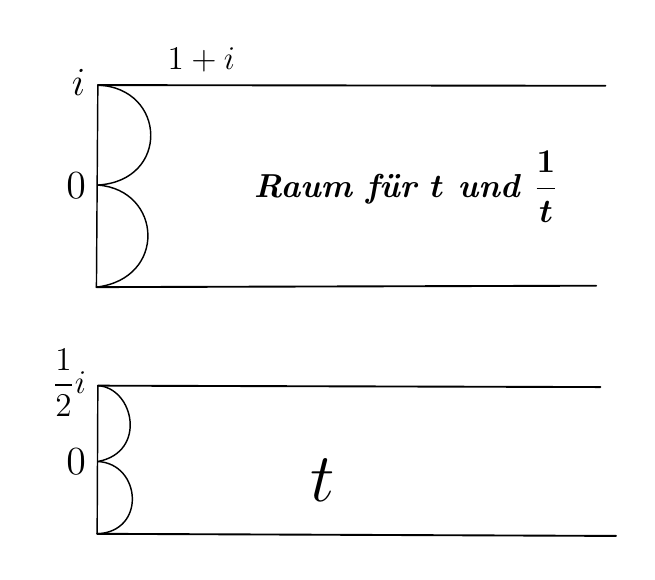
\begin{tikzpicture}[x=.009cm,y=-.009cm,line cap=round,line join=round]
\path[use as bounding box] (15,25) rectangle (860,765);
\draw[line width=.68pt] (114,106)--(830,107);
\draw[line width=.52pt] (114,106)--(112,391);
\draw[line width=.68pt] (112,391)--(817,389);
\draw[line width=.52pt] (114,106)..controls (211,110) and (216,241)..(114,247);
\draw[line width=.52pt] (114,247)..controls (205,254) and (212,379)..(112,391);
\draw[line width=.68pt] (114,530)--(823,532);
\draw[line width=.52pt] (114,530)--(113,739);
\draw[line width=.68pt] (113,739)--(845,742);
\draw[line width=.52pt] (114,530)..controls (165,533) and (184,624)..(114,637);
\draw[line width=.52pt] (114,637)..controls (175,640) and (183,736)..(113,739);
\node[anchor=east,inner sep=0pt,font=\Large] at (97,102) {$i$};
\node[anchor=south,inner sep=0pt,font=\large] at (260,89) {$1+i$};
\node[anchor=east,inner sep=0pt,font=\Large] at (98,248) {$0$};
\node[anchor=center,inner sep=0pt,font=\large\bfseries\itshape] at (549,249) {Raum für $\boldsymbol{t}$ und $\boldsymbol{\dfrac1t}$};
\node[anchor=east,inner sep=0pt,font=\large] at (98,526) {$\dfrac12 i$};
\node[anchor=east,inner sep=0pt,font=\Large] at (98,637) {$0$};
\node[anchor=center,inner sep=0pt,font=\Huge] at (431,663) {$t$};
\end{tikzpicture}
}\end{center}

\[
\left(\frac{qt}{pt}\right)^{2}
\]
bezogen sind, welche positiven reellen Bestandtheil haben. Es handelt sich hierbei um die Function $k'$ der neueren Theorie, welche den sogen. complementären Modul des elliptischen Integrals erster Gattung in seiner Abhängigkeit vom Periodenquotienten darstellt. In der a.\,a.\,O. von \textsc{Gauss} angegebenen Gleichung:

\[
\left(\frac{qt}{pt}\right)^{2} = A
\]
ist übrigens $A$ als complexe Zahl mit einem absoluten Betrage $\leqq 1$ an\-zunehmen; andrenfalls müsste man den Bereich der $t$-Ebene in geeigneter Weise verdoppeln.

Hiermit hängen auch die Angaben zu Anfang des Fragmentes [3] unmittelbar zusammen. Es ist dazu nur noch zu bemerken, dass man sogar alle Lösungen der Gleichung:

\[
\left(\frac{qt}{pt}\right)^{2} = A^{2}
\]
erhält, falls man in der angegebenen Weise alle der Bedingung $\alpha\delta - 4\beta\gamma = 1$ genügenden ganzen Zahlen $\alpha, \beta, \gamma, \delta$ zulässt.

Nicht direct im Zusammenhang hiermit stehen die gegen Ende des Fragmentes [3] angeschlossenen Bemerkungen über die Berechnung von $B = \dfrac{q(\frac13 t)}{p(\frac13 t)}$ aus $A$. Die hier mitgetheilte Gleichung hat \textsc{Jacobi} späterhin als Modulargleichung für Transformation dritten Grades wiedergefunden, und sie tritt bekanntlich in besonders eleganter (irrationaler) Gestalt auch bei \textsc{Legendre} auf.

Die am Schlusse des Fragmentes beigefügten numerischen Angaben sind übrigens in den letzten Decimalstellen mehrfach ungenau.

Den Zusammenhang zwischen der Theorie der Modulfunctionen und der Arithmetik der binären quadratischen Formen von negativer Determinante hat \textsc{Gauss} frühzeitig erkannt. Neben Art.~17 ist für die Reductionstheorie der Formen namentlich das Fragment [2] von Wichtigkeit. Dabei beachte man insbesondere die Schlusszeile; \textsc{Gauss} hat daselbst ausgesprochen, dass die Reductionstheorie keineswegs an die Voraussetzung ganzzahliger oder rationaler Coefficienten gebunden ist. \hfill \textsc{Fricke}.

\end{document}
